\subsection{PCR Testing and Behavioral Response}
\label{subsec:pcr_testing_and_behavioral_response}

 \comment[id=K]{@Janos: Read this}

After showing how we calibrate rapid test demand and the share of detected cases, this
section describes the remaining parameters for our testing model. Refer to
Section~\ref{sub:testing} for a description of the full testing model.

% share of tests for symptomatics
From the share of detected cases and the number of infections we arrive at the number of
positive PCR tests in our model. A share of these positive tests is given to symptomatic
individuals ($\chi_{symptom,\:t}$). This share is calibrated from German data on case
characteristics \citep{RKICaseCharacteristics} and shown in
Figure~\ref{fig:share_pcr_to_symptomatic}. We keep $\chi_{symptom,\:t}$ constant after
Christmas because the RKI data does not include if a PCR test was done to confirm a
positive rapid test and this share is used for PCR test demand without prior rapid test
indication

\begin{figure}
    \centering
    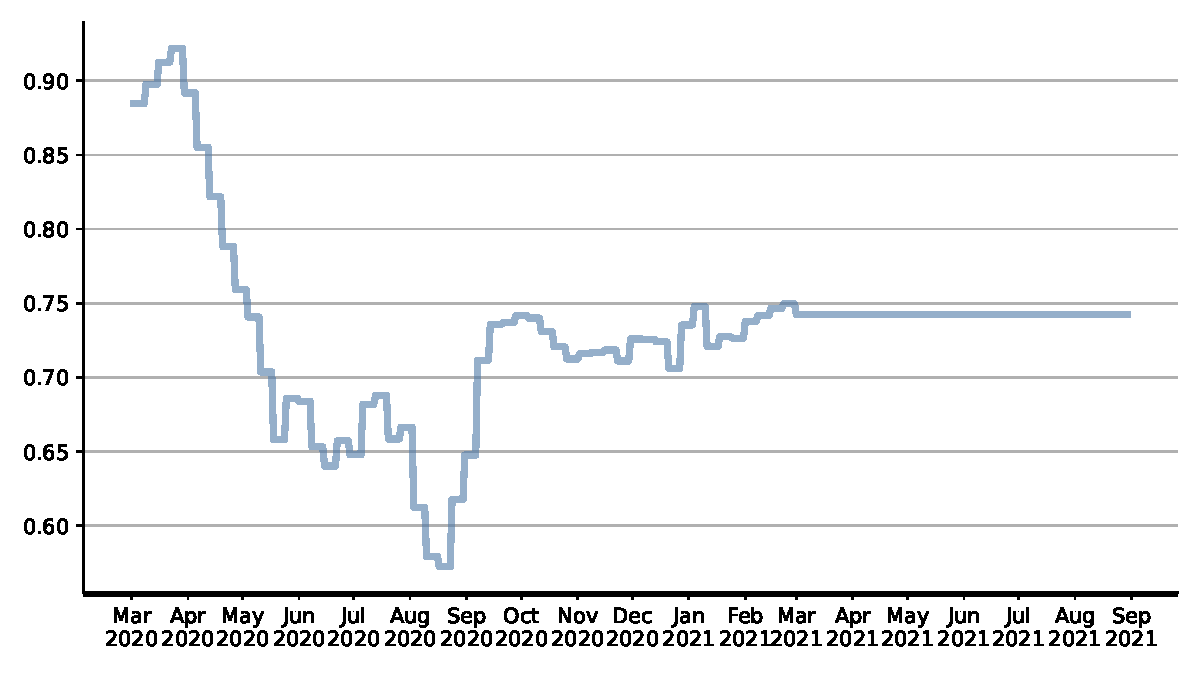
\includegraphics[width=0.5\textwidth]{figures/results/figures/data/testing/used_share_of_pcr_tests_going_to_symptomatics}
    \caption{Share of Positive PCR Tests Administered to Symptomatic Individuals}
    \label{fig:share_pcr_to_symptomatic}
    \floatfoot{\noindent \textit{Note:} The share of positive PCR tests that are
    administered to symptomatic individuals ($\chi_{symptom,\:t}$). Since it was not
    recorded for every case if the person was symptomatic or not we take the midpoint
    between the upper and lower bound. We keep the share constant after Christmas because
    the RKI data does not include if a PCR test was done to confirm a positive rapid test
    and this share is used for PCR test demand without prior rapid test indication.}
\end{figure}

% time until test result
PCR tests take one to four days until their result is revealed to the individual
($\gamma_{PCR,\:d}$). Relying on the ARS data \citep{ARS2020} we calculate that 33\% of
individuals receive the test result after one day, 50\% after two days, 10\% after three
days and 7\% after four days.

% share with positive rapid test requesting pcr
To model the demand for PCR tests through rapid tests, we only need the share of
individuals that seek a PCR test to confirm a positive rapid test result
($\chi_{confirmation}$). We calibrate this from \citet{Betsch2021} who asked this
hypothetical question in March of 2021. There 82\% of Germans reported that they would
follow up on a positive rapid test with a PCR test.

% Behavioral Response ------------------------------------------------------------------

Lastly, we need to set the parameters that decide how individuals reduce their contacts
after certain events, $\tau$. We distinguish between the reduction in household contacts
(which are harder to avoid) and non household contacts. There are three events which
trigger potential contact reductions: showing symptoms of CoViD-19, having received a
positive rapid test and having received a positive PCR test. The only survey data we are
aware of on this is \citet{Betsch2021} where 85\% of individuals claimed they
would isolate and restrict their contatcs after a positive rapid test. We assume this
reduction for non household contacts. As household contacts are much more difficult to
avoid, we assume that they are only reduced by 30\%. We assume the same behavior for
individuals that develop symptoms. Lastly, we assume the response to a positive PCR test
to be stronger than in the other two cases and set the reduction of non household
contacts to 95\% and the reduction of household contacts to 50\%.

\FloatBarrier